\documentclass[11pt]{article}\usepackage{knitr}

%AMS-TeX packages
\usepackage{amssymb,amsmath,amsthm} 
%geometry (sets margin) and other useful packages
\usepackage[margin=1in]{geometry}
\usepackage{graphicx, ctable, booktabs}
\usepackage{color}
\usepackage{listings}
\usepackage{ltablex, calc, enumerate, multirow, float, soul, paralist}
\usepackage{hyperref}
\usepackage{longtable, pdflscape, textcase}
\usepackage[backend=bibtex, natbib=true]{biblatex}
\addbibresource{references/refs.bib}
\IfFileExists{upquote.sty}{\usepackage{upquote}}{}

\begin{document}









\setlength{\parskip}{3ex}
\setlength{\parindent}{0pt}

\title{Putting Down Roots: A Graphical Exploration of Community Attachment}
\author{Andee Kaplan, Eric Hare}

\maketitle

\begin{abstract}
In this paper, we explore the relationships that individuals have with their communities. This work was prepared as part of the ASA Data Expo ’13 sponsored by the Graphics Section and the Computing Section, using data provided by the Knight Foundation Soul of the Community survey. The Knight Foundation in cooperation with Gallup surveyed 43,000 people over three years in 26 communities across the United States with the intention of understanding the association between community attributes and the degree of attachment people feel towards their community. These include the different facets of both urban and rural communities, the impact of quality education, and the trend in the perceived economic conditions of a community over time. We begin by focusing on the choices made in producing the visualizations and technical aspects of how they were created. We will explain the development and use of web-based interactive graphics, including an overview of the R package shiny and the JavaScript library D3. Then we describe the stories about community attachment that unfolded from our analysis.
\end{abstract}

\clearpage

\setcounter{page}{1}
\section{Introduction}

This work was part of the American Statistical Association's Data Exposition 2013 sponspored by the Knight Foundation and the Graphics/Computing Section of the ASA.

\subsection{Data}
The dataset comes from the Knight Foundation's `Soul of the Community' project. For this project, the Knight Foundation in conjunction with Gallup collected surveys from 43,000 people over three years in 26 U.S. communities. This was not a random sample of communities across the United States, but rather they were chosen as places that the Knight Foundation was already active. The survey contains raw responses as well as derived metrics that we used to gain insight into what makes a community thrive. The metrics we used can be found in Table~\ref{tab:metrics}.

\begin{table}[H]
\centering
\begin{tabular}{l l}
\hline
Metrics & \\
\hline
Community Attachment (1-5) & Social Offerings \\
Safety & Social Capital \\
Education & Basic Services \\
Leadership & Civic Involvement \\
Aesthetics & Openness \\
Economy &  \\
\hline
\end{tabular}
\caption{\label{tab:metrics} The metrics used from the Knight Foundation Soul of the Community survey. All metrics are on a 1-3 scale except for Community Attachment, which is on a scale of 1-5.}
\end{table}

\subsection{Philosophy}
The goal of our work is to facilitate understanding of why people feel attachment to their communities through the use of an interactive and web-based approach. Specifically, we took the point of view of a community planner, either from one of the communities in the study or from a community in the same region or a similar urbanicity. By putting the user in the driver seat of their own experience, we allow the user to apply the conclusions of their interaction to their own situation.


\section{Technology}

In order to explore the dataset, we first created an interactive tool called {\it CommuniD3} (available at \url{http://glimmer.rstudio.com/andeek/DataExpo2013}) to facilitate the emergence of interesting or descriptive patterns. The construction and design of this tool are detailed in the following sections.

\subsection{Description and Design}
CommuniD3 is comprised of three pieces, \begin{inparaenum}[(1)]
\item Side panel, 
\item Map Panel, and
\item Plot panel,
\end{inparaenum}
as seen in Figure~\ref{fig:tool}.
As the user interacts with each piece, the remaining portions of the interface update to reflect the interaction. In this way we have built an interactive graphic, rather than an animation.

\begin{figure}[H]
\centering
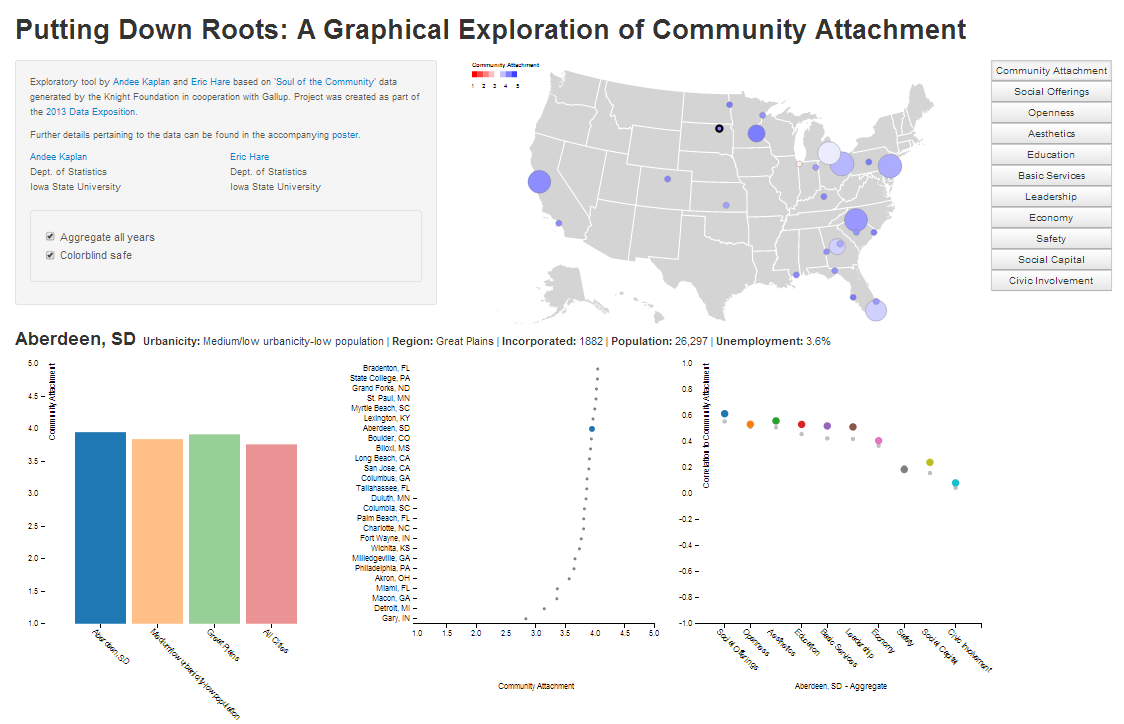
\includegraphics[width=\textwidth]{images/tool.png}
\caption{\label{fig:tool} The components that make up CommuniD3, (1) Side panel, (2) Map panel, and (3) Plot panel.}
\end{figure}

\paragraph{Side panel} The side panel houses two features. The first is the ability to look at the data for individual years versus aggregated across all three years. In this way we are able to explore attitude changes across the three years surveyed as well as overarching trends in the regions and urbanicities. The second is a colorblind friendly option that uses blue on the map rather than green to accomodate more users.

\paragraph{Map panel} The map panel is the central piece of the application. A bubble chart of the 26 communities surveyed are plotted geographically on a map of the United States. The size of each dot represents how many surveys were received for the time period selected and the color of each dot corresponds to the average value for each community in the time period selected for the metric selected. There is a right panel that allows for the user to change which metric is displayed. Additionally, each community is clickable. On click, basic information about that community is displayed below the map panel and the plot panel is updated to refect the community that is clicked. It is our goal for a community planner to be able to start with the map panel and find a community that was surveyed that corresponds to the community they are interested about, or one that is nearby, as a means to delve into the driving factors of community attachment.

\paragraph{Plot panel} The plot panel is a set of three linked plots that detail three aspects of the dataset. The first plot is a bar graph showing the average value of the metric selected for the year range selected for the community selected as well as for its region and its urbanicity. For example, if Detroit, MI is the community selected, then the region would be Rust Belt and the urbanicity ``Very high urbanicity-very large population''. There is also a 4th bar in the chart that represents the aggregation of all the communities serves as a reference. While the bar chart is a plot that shows surface information, its true purpose is to control the information displayed in the other two plots. As the user clicks on the bars, the second two plots will display information pertaining to the level selected (either region, urbanicity, or the whole dataset). The middle plot is an ordered dot plot displaying the average value for the metric selected for all communities with the level selected in the bar chart highlighted. See Figure~\ref{fig:dots} for an example of the dfferent highlighting available. Finally, the third plot is a plot of correlations between each metric and community attachment for the level of aggregation (year and community/region/urbanicity) selected. There is a reference level in the background that displays the correlation for every survey aggregated to ease comparison for the user. The three plots are linked in such a way that selection through clicking in one plot will affect all three plots and potentially the map panel. In this manner, the user can truly drive their experience and take ownership of their analysis.

\begin{figure}[H]
\centering
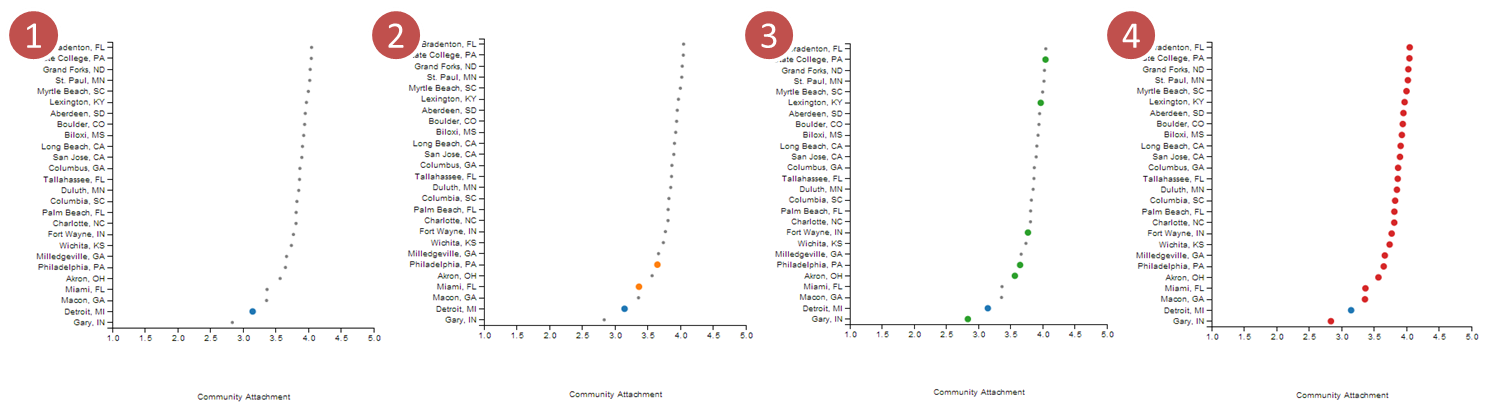
\includegraphics[width=\textwidth]{images/dots.png}
\caption{\label{fig:dots} Examples of the different types of highlighting available in the ordered dot plot from the plot panel. The highlighting corresponds to (1) community selection, (2) region selection, (3) urbanicity selection, and (4) all community selection. In this example, Detroit, MI has been selected to display the values of community attachment for all three years, 2008-2010.}
\end{figure}

\subsection{The Shoulders of Giants}
We were able to incorporate several pioneering technologies in the creation of our application that allowed us to find insights in the dataset.

\paragraph{Shiny}
Shiny \cite{rs-shiny} is an {\tt R} package created by RStudio that enables {\tt R} users to create an interactive web application that utilizes {\tt R} as the background engine. Through default methods to build user interface elements in HTML and a handle to the server side code, Shiny is a simple way to turn {\tt R} code into a website. 

In CommuniD3, Shiny is used as the framework upon which the application sits. Shiny allows us to manipulate the underlying dataset using {\tt R} on the server before passing it to the client side and used in displaying the plots.

\paragraph{D3}
D3 \cite{mb-d3} stands for ``Data Driven Documents" and is a JavaScript library developed and maintained by Mike Bostock with the  purpose of visualizing and interacting with data in a web-based interface. It is freely available from \url{http://www.d3js.org}. The library facilitates manipulation of HTML elements, SVG (scalable vector graphics), and CSS (cascading style sheets) with the end goal of rendering animations and providing user interactions that are tied to the underlying data. The key idea behind the library is that Document Object Model elements are completely determined by the data. The Document Object Model (DOM) is a convention for representing and interacting with objects in HTML, XHTML and XML. So, rather than adding elements to a web page to be viewed by users, D3 allows users to see and interact with graphical representations of their data in a web framework. 

We used D3 and JavaScript to create the visualizations as well as control all the user interaction with the application. The graphics and user interface are all stored entirely on the client side, allowing for seemless transitions of the graphics. See Figure~\ref{fig:D3shiny} for a diagram of the ways Shiny and D3 are used in CommuniD3.

\begin{figure}[H]
\centering
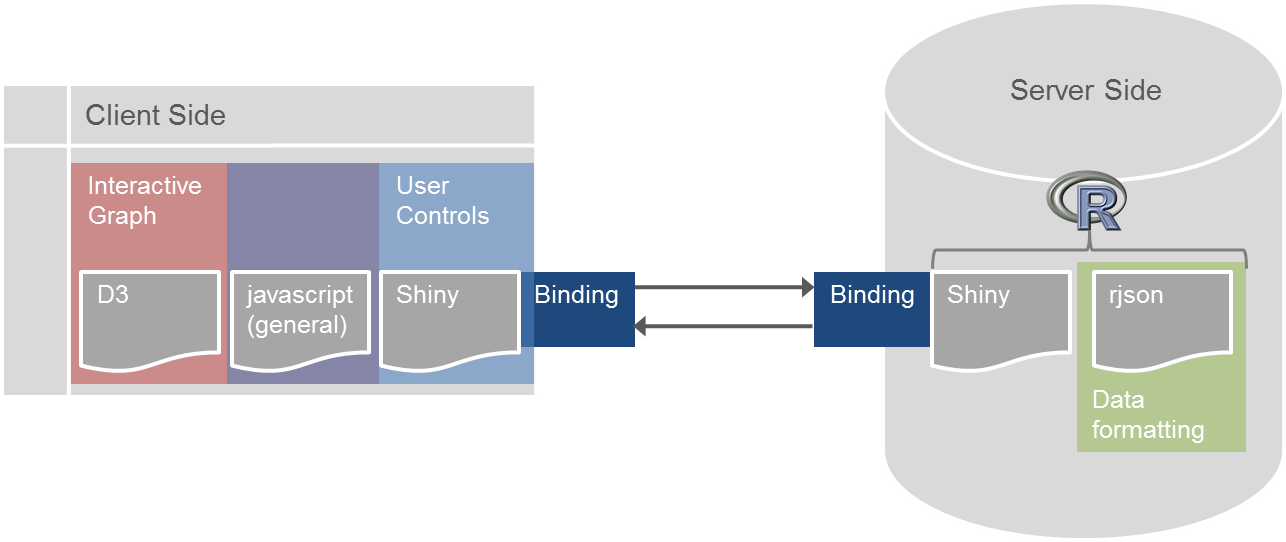
\includegraphics[width=\textwidth]{images/D3shiny.png}
\caption{\label{fig:D3shiny} Diagram of the uses of D3 and Shiny in CommuniD3, specifically focusing on client versus server utilization.}
\end{figure}

\paragraph{Other Packages}
We also leveraged other {\tt R} packages to help with data manipulation. We used plyr \cite{plyr}, reshape2 \cite{reshape2}, and rjson \cite{rjson} to split and aggregagate metric values according to the levels selectable by the user before passing the data to the client side in the JSON format. 

For subsequent analysis after using CommuniD3 we used the {\tt R} packages ggplot2 \cite{ggplot2} and maps \cite{maps} to dive deeper into the interesting findings from the application.


\subsection{Why?}
During the creation of CommuniD3, we found it useful to stop and ask, ``Why?'' This process enabled the type of introspection necessary to help ensure usability and relevance in a project of this type.

\paragraph{Interactive}
Why interactive? In order to discover what the data has to tell the world. In the words of John Tukey, "Exploratory data analysis is detective work - numerical detective work - or counting detective work - or \emph{graphical detective work}." \cite{tukey77} Dynamic, interactive visualizations can empower people to explore the data for themselves as well as encourage engagement with the data in a way that static visualizations cannot.

\paragraph{Linked Plots}
Why linked plots? Linking multiple visualizations shows different aspects of a complex data set and helps highlight relationships. By allowing actions in one plot to affect elements in other plots, comparisons are made easy for the user without requiring much memorization. This aids in pattern finding by avoiding taxation of the user's brain through memorization.

\paragraph{Web-based}
Why web-based? A web-based application is platform-independent and allows the user to employ the tool without any software to download. Additionally, by building an application that works on all modern browsers and operating systems, there are no limitations on who can use the tool. Finally, automatic feature additions and bug fixes can be completed transparently to the user.


\section{Stories}

We elected to divide our analysis using two primary factors. The first is the geographic region the community is located in, and the second is the urbanicity of the particular community. Urbanicity is a census designation which was provided in the dataset, while regions were determined by us. The regions are a rough guideline and do not correspond to any commonly used or accepted regional boundaries. They were merely a method we used to cluster communities into more-alike regions in terms of geography and culture. The interactive tool was then used to help us discover a story in the data for each of the five regions. A map of the regions is displayed in Figure \ref{fig:region_map}.

\begin{knitrout}
\definecolor{shadecolor}{rgb}{0.969, 0.969, 0.969}\color{fgcolor}\begin{figure}[H]


{\centering 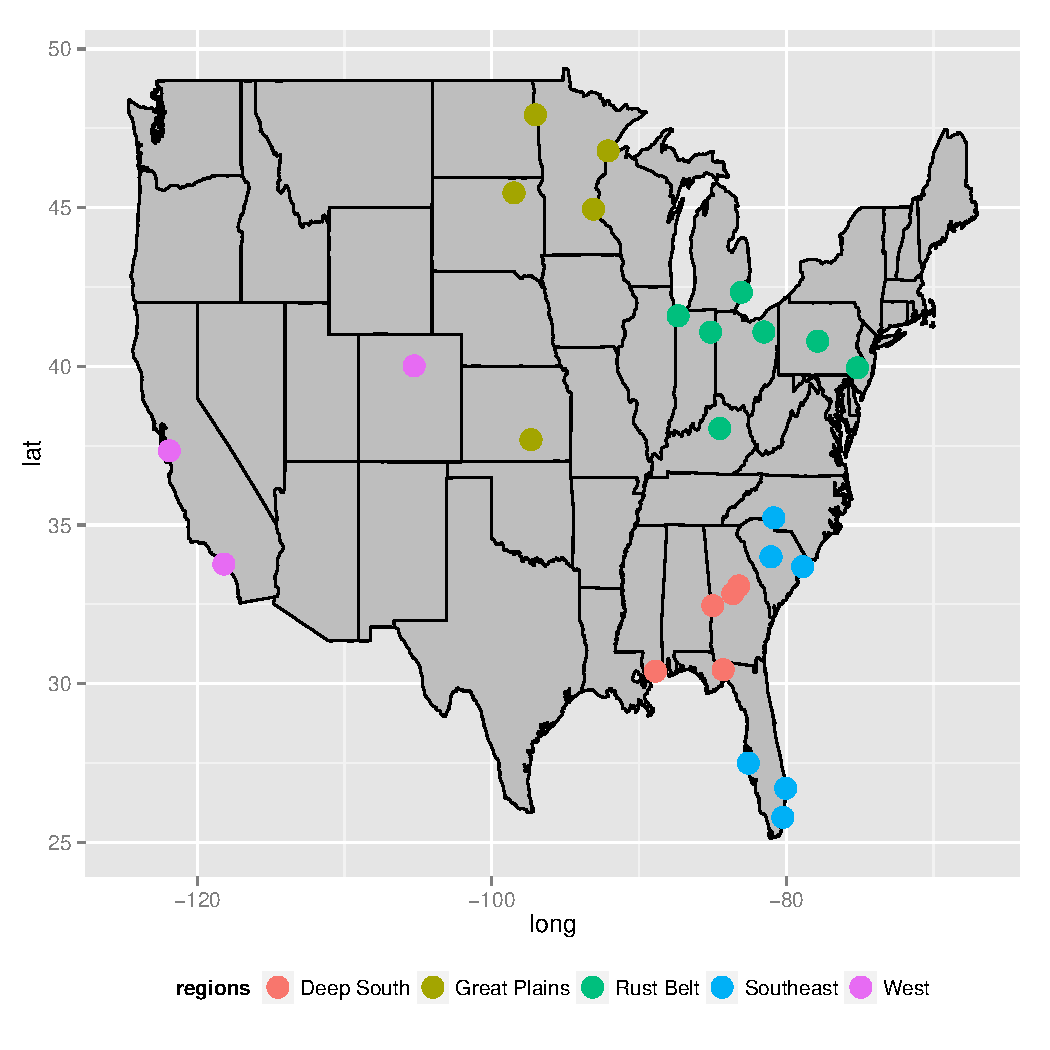
\includegraphics[width=\textwidth]{figure/region_map} 

}

\caption[Map of the five regions to which we assigned the communities]{Map of the five regions to which we assigned the communities.\label{fig:region_map}}
\end{figure}


\end{knitrout}


\subsection{Great Plains}
The five communities comprising the Great Plains are Grand Forks, ND, Duluth, MN, Aberdeen, SD, Saint Paul, MN, and Wichita, KS. Through use of the interactive tool, we quickly discovered that the individuals in this region tended to rate the quality of education in the community more highly. In Table \ref{tbl:edu_table}, the top eight communities by the Education Metric are displayed. It can be seen that the Great Plains region includes three of the top four, and four of the top eight communities in terms of Education. Grand Forks, ND in particular has the highest average response for this metric amongst all communities. This is perhaps not too surprising given the presence of the University of North Dakota in this community.

% latex table generated in R 3.0.2 by xtable 1.7-1 package
% Thu Feb 13 11:32:17 2014
\begin{table}[ht]
\centering
\begin{tabular}{llr}
  \hline
Region & Community & Education \\ 
  \hline
Great Plains & Grand Forks, ND & 2.4001 \\ 
  Rust Belt & State College, PA & 2.3648 \\ 
  Great Plains & Aberdeen, SD & 2.2554 \\ 
  Great Plains & St. Paul, MN & 2.1318 \\ 
  West & Boulder, CO & 2.1294 \\ 
  Rust Belt & Philadelphia, PA & 2.1006 \\ 
  Deep South & Tallahassee, FL & 2.0948 \\ 
  Great Plains & Duluth, MN & 2.0927 \\ 
   \hline
\end{tabular}
\caption{Top Six Communities by the Education Metric.} 
\label{tbl:edu_table}
\end{table}



We can visualize the distribution of the Education metric values for each of the Great Plains communities compared to all other communities. Histograms of these values are displayed in Figure \ref{fig:gp_one}. With the exception of Wichita, KS, the Great Plains communities have more responses in the higher values when compared with communities in other regions. This is most visible in both Grand Forks, ND and Aberdeen, SD.

\begin{knitrout}
\definecolor{shadecolor}{rgb}{0.969, 0.969, 0.969}\color{fgcolor}\begin{figure}[H]


{\centering 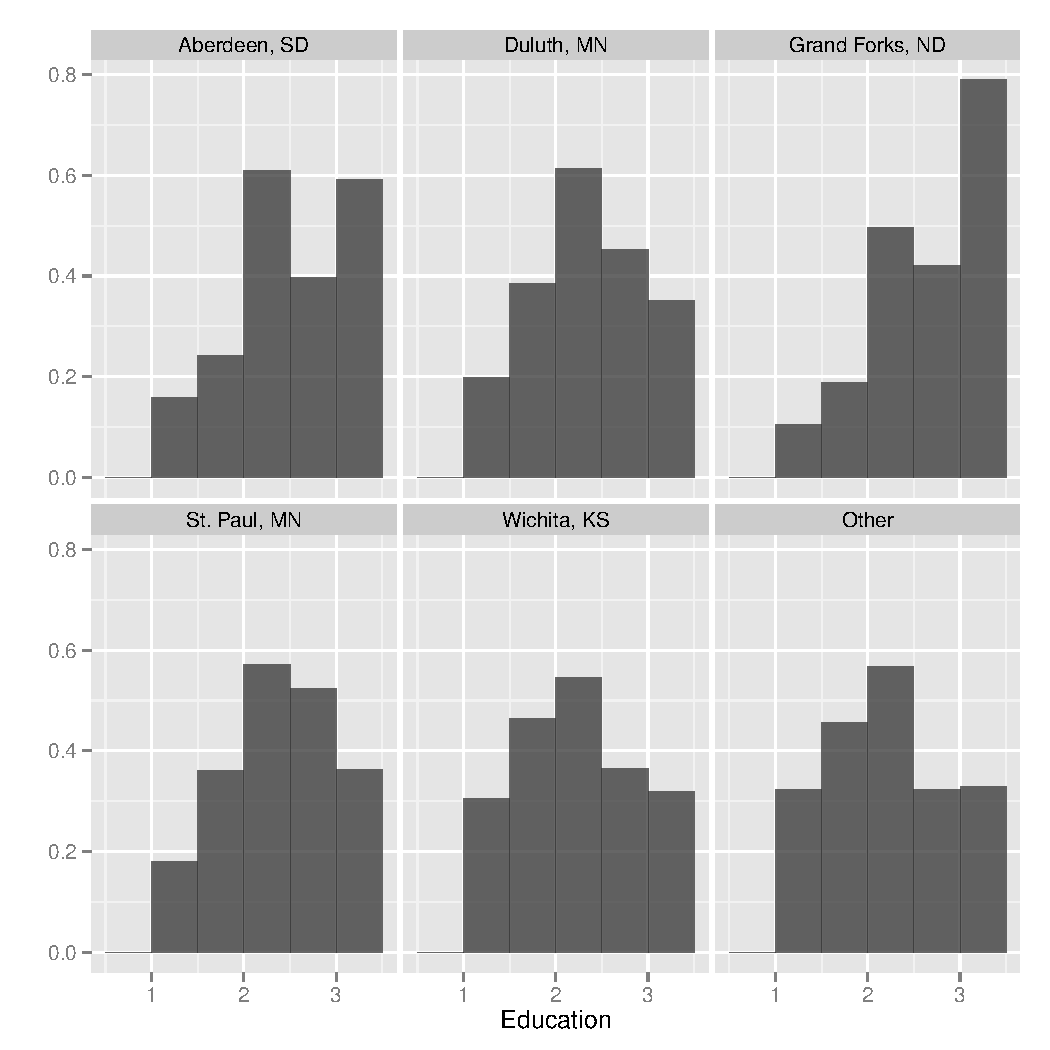
\includegraphics[width=\maxwidth]{figure/gp_one} 

}

\caption[Histograms of responses to Education for the five Great Plains communities, and all other communities aggregated]{Histograms of responses to Education for the five Great Plains communities, and all other communities aggregated.\label{fig:gp_one}}
\end{figure}


\end{knitrout}


What might be more surprising is illustrated in Table \ref{tbl:cce_table}; the Great Plains region itself has the largest overall Community Attachment among the five regions. As it turns out, the correlation of the Education metric to the Community Attachment metric in the Great Plains is 0.49. This compares to a correlation of 0.46 in the communities outside the Great Plains. This correlation is illustrated in Figure \ref{fig:gp_two}. The mean response for Community Attachment is plotted versus the mean response for Education in each of the Great Plains communities, and all other communities aggregated. The big dots represent the data aggregated over all years, while the smaller dots represent 2008, 2009, and 2010. A pretty strong relationship between Education and Community Attachment can be observed, but with one notable exception: Saint Paul, MN. Saint Paul has a much higher Community Attachment given its value for Education than what would be expected by observing the other communities. This is likely due Saint Paul's size and cultural presence, which may contribute to other factors which lead to a high sense of Community Attachment.

% latex table generated in R 3.0.2 by xtable 1.7-1 package
% Thu Feb 13 11:32:23 2014
\begin{table}[ht]
\centering
\begin{tabular}{lr}
  \hline
Region & Community Attachment \\ 
  \hline
Deep South & 3.7358 \\ 
  Great Plains & 3.9165 \\ 
  Rust Belt & 3.5677 \\ 
  Southeast & 3.8086 \\ 
  West & 3.9150 \\ 
   \hline
\end{tabular}
\caption{The average value for the Community Attachment metric in each of the five regions.} 
\label{tbl:cce_table}
\end{table}



\begin{knitrout}
\definecolor{shadecolor}{rgb}{0.969, 0.969, 0.969}\color{fgcolor}\begin{figure}[H]


{\centering 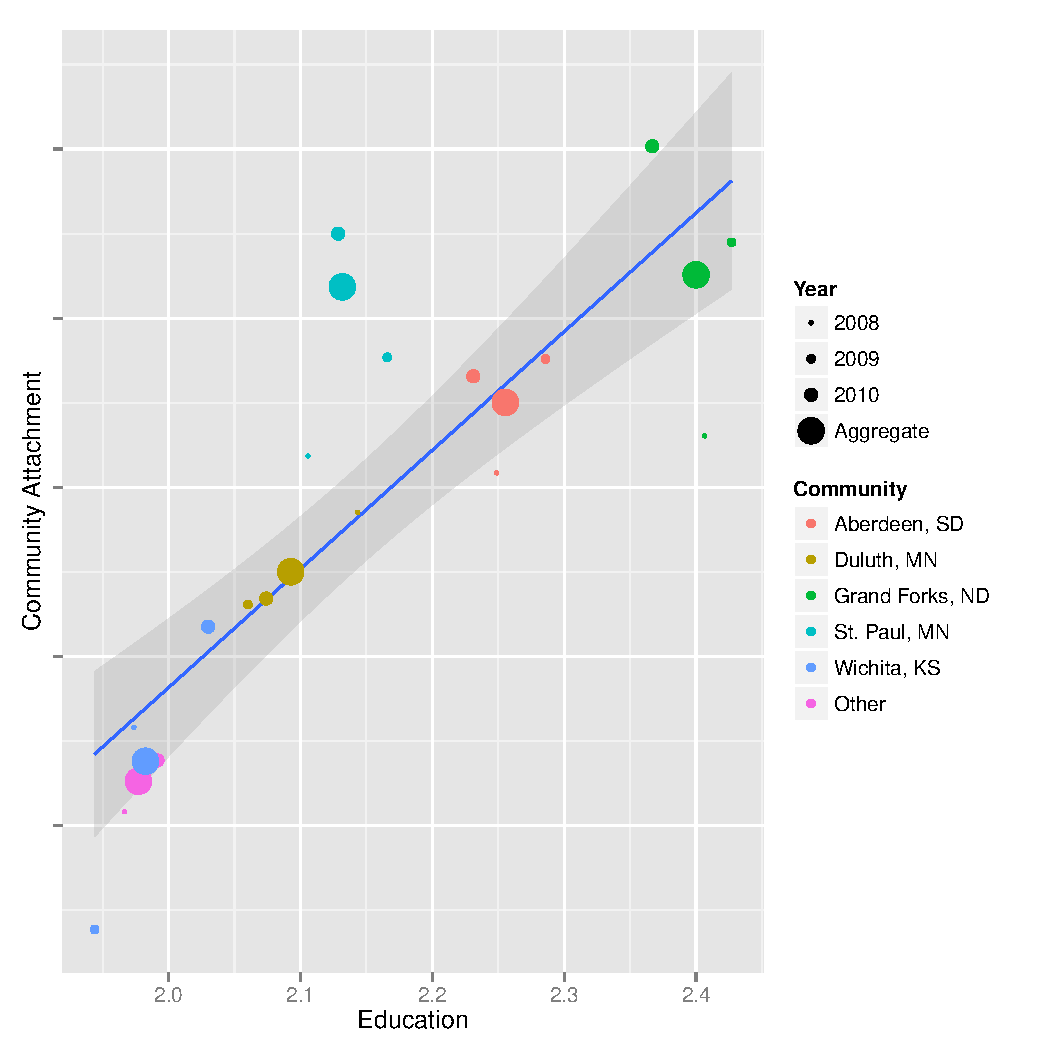
\includegraphics[width=\maxwidth]{figure/gp_two} 

}

\caption[Mean Community Attachment value versus mean Education value]{Mean Community Attachment value versus mean Education value. The size of the dots represent the year, while the color represents the community.\label{fig:gp_two}}
\end{figure}


\end{knitrout}



\subsection{West}
We also focused our analysis on the Urbanicity designations of the communities. We were interested in seeing if some different metrics may contribute to a sense of community attachment depending on the community's urbanicity. In the West region, which comprises Boulder, CO, San Jose, CA, and Long Beach, CA, we found some evidence of an urbanicity-specific metric correlated with attachment.

Table \ref{tbl:open_table} displays the top five communities by the Openness Metric. First, it can be seen that the three communities comprising the West Region are each in the top five for Openness. Second, Boulder and Long Beach each have the urbanicity of "Very high urbanicity-medium population". These communities consist of a relatively modest population, but where most of whom live in the urban core of the city. Figure \ref{fig:west_one} displays a two-dimensional bin plot of Community Attachment versus Openness, displaying only the communities with the designation "Very high urbanicity-medium population". Areas of darker red have a higher frequency of responses than those that are white. Notice that both Boulder and Long Beach tend to have more respondents indicating a high Community Attachment and a high Openness. By comparison, Akron, OH, and Gary, IN, two communities in the Rust Belt region with the same urbanicity, have much lower ratings on both of these scales. Bradenton, FL has many citizens highly attached to the community, but somewhat lower ratings for Openness compared to Boulder and Long Beach. Ultimately, it would seem that communities in the West region with this urbanicity designation place a higher value on the Openness of their community than do other communities of similar size in the rest of the country.

% latex table generated in R 3.0.2 by xtable 1.7-1 package
% Thu Feb 13 11:32:23 2014
\begin{table}[ht]
\centering
\begin{tabular}{lllr}
  \hline
Community & Region & Urbanicity & Openness \\ 
  \hline
Long Beach, CA & West & Very high urbanicity-medium population & 1.9496 \\ 
  San Jose, CA & West & Very high urbanicity-large population & 1.8761 \\ 
  St. Paul, MN & Great Plains & Very high urbanicity-large population & 1.8758 \\ 
  State College, PA & Rust Belt & Medium/low urbanicity-low population & 1.8659 \\ 
  Boulder, CO & West & Very high urbanicity-medium population & 1.8361 \\ 
   \hline
\end{tabular}
\caption{Top Five Communities by the Openness Metric.} 
\label{tbl:open_table}
\end{table}



\begin{knitrout}
\definecolor{shadecolor}{rgb}{0.969, 0.969, 0.969}\color{fgcolor}\begin{figure}[H]


{\centering 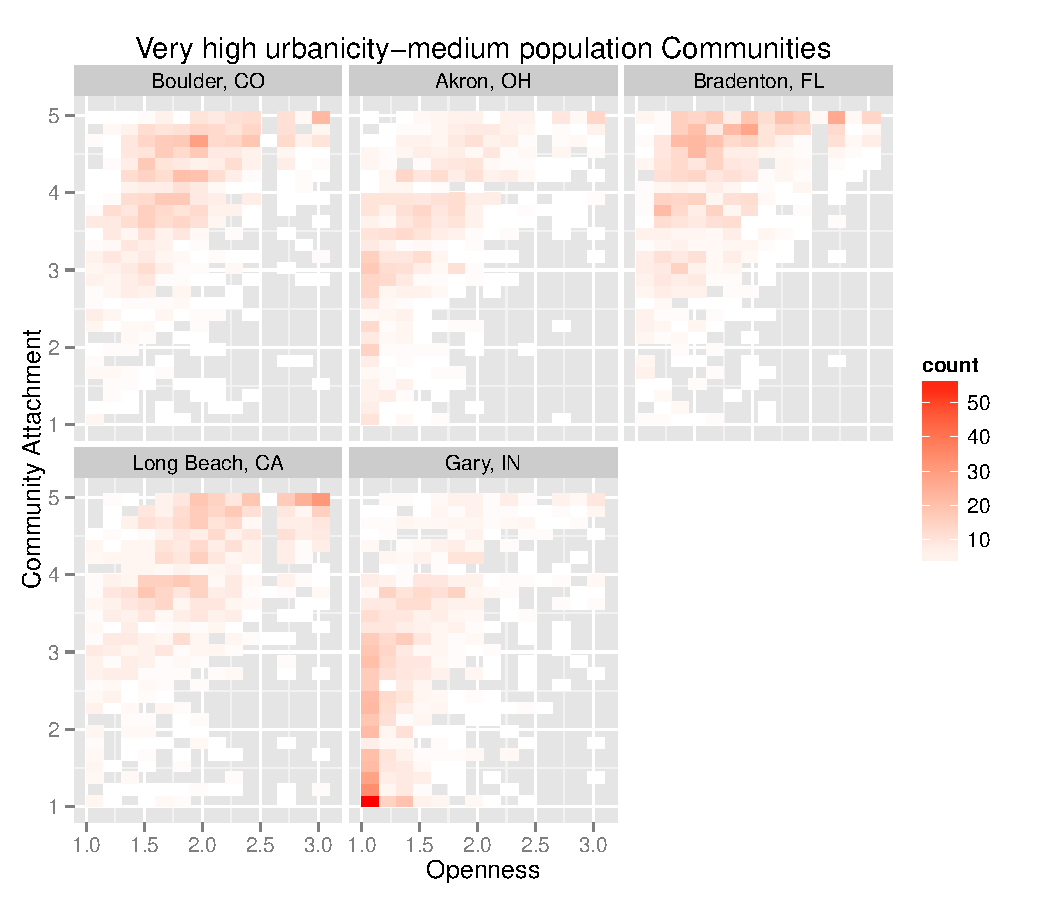
\includegraphics[width=\maxwidth]{figure/west_one} 

}

\caption[Binned density plot of responses for Openness and Community Attachment among the five communities with Very high urbanicity-medium population designations]{Binned density plot of responses for Openness and Community Attachment among the five communities with Very high urbanicity-medium population designations.\label{fig:west_one}}
\end{figure}


\end{knitrout}


\subsection{Deep South}
Exploring trends in the Deep South communities of Macon, GA, Milledgeville, GA, Columbus, GA, Tallahassee, FL, and Biloxi, MS quickly suggested that residents of these communities were displeased with the Safety of the community. In 2008, Macon and Columbus ranked 3rd and 4th worst respectively among all 26 communities in terms of Safety. By 2010, the situation degraded further, as Macon declined to the overall worst Safety rating, while Milledgeville ranked 3rd worst, and Columbus remained the 4th worst. Biloxi was a notable exception, however, ranking 8th best in 2010. Biloxi also exceeded its fellow Deep South communities in terms of Social Offerings, ranking 2nd best amongst all communities in each of the three years the survey was conducted, and by far the best amongst the communities in the Deep South.

As it turns out, Biloxi also had the highest overall Community Attachment rating in the Deep South. Figure \ref{fig:ds_one} displays the average rating from 2008 to 2010 in terms of Safety, Social Offerings, and Community Attachment. Biloxi is highlighted in red, the other Deep South communities are highlighted in blue, and the rest of the communities in gray. The stark difference in Biloxi compared with the rest of the Deep South is readily apparent, and helps to explain why Community Attachment is quite high in Biloxi.

\begin{knitrout}
\definecolor{shadecolor}{rgb}{0.969, 0.969, 0.969}\color{fgcolor}\begin{figure}[H]


{\centering 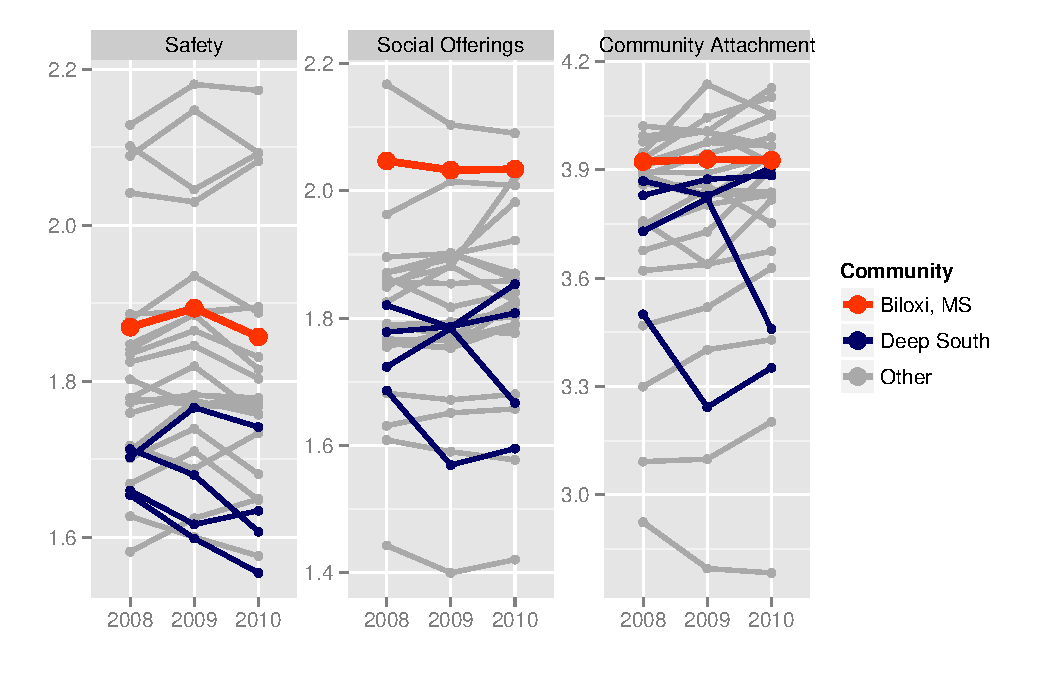
\includegraphics[width=\maxwidth]{figure/ds_one} 

}

\caption[Responses across the three years for Safety, Social Offerings, and Community Attachment]{Responses across the three years for Safety, Social Offerings, and Community Attachment.\label{fig:ds_one}}
\end{figure}


\end{knitrout}


\subsection{Southeast}
In the Deep South, we saw some evidence suggesting Biloxi's high rating for Social Offerings may be contributing to a strong sense of attachment in that community. Nowhere is this phenomenon more prominent than in the Southeast region, where Myrtle Beach, SC resides. Myrtle Beach is the 5th most attached community amongst all communities in the dataset. However, Myrtle Beach does no better than 13th in all other metrics with the exception of Social Offerings, where it is ranked 1st. In other words, residents of Myrtle Beach felt the Social Offerings in their community were very strong, while most other metrics, including Aesthetics, Openness, Safety, and Education were poor. Figure \ref{fig:southeast_one} illstruates this phenomenon with a parallel coordinate plot. The mean value for all metrics is displayed for each of the communities, with Myrtle Beach highlighted in green, and other Southeast communities highlighted in blue. The metrics are sorted from high to low by the average value for each metric amongst all the communities. Notice that Myrtle Beach fairly closely tracks the rest of the communities in all metrics except for Social Offerings, where a sizable ``jump'' can be observed.

\begin{knitrout}
\definecolor{shadecolor}{rgb}{0.969, 0.969, 0.969}\color{fgcolor}\begin{figure}[H]


{\centering 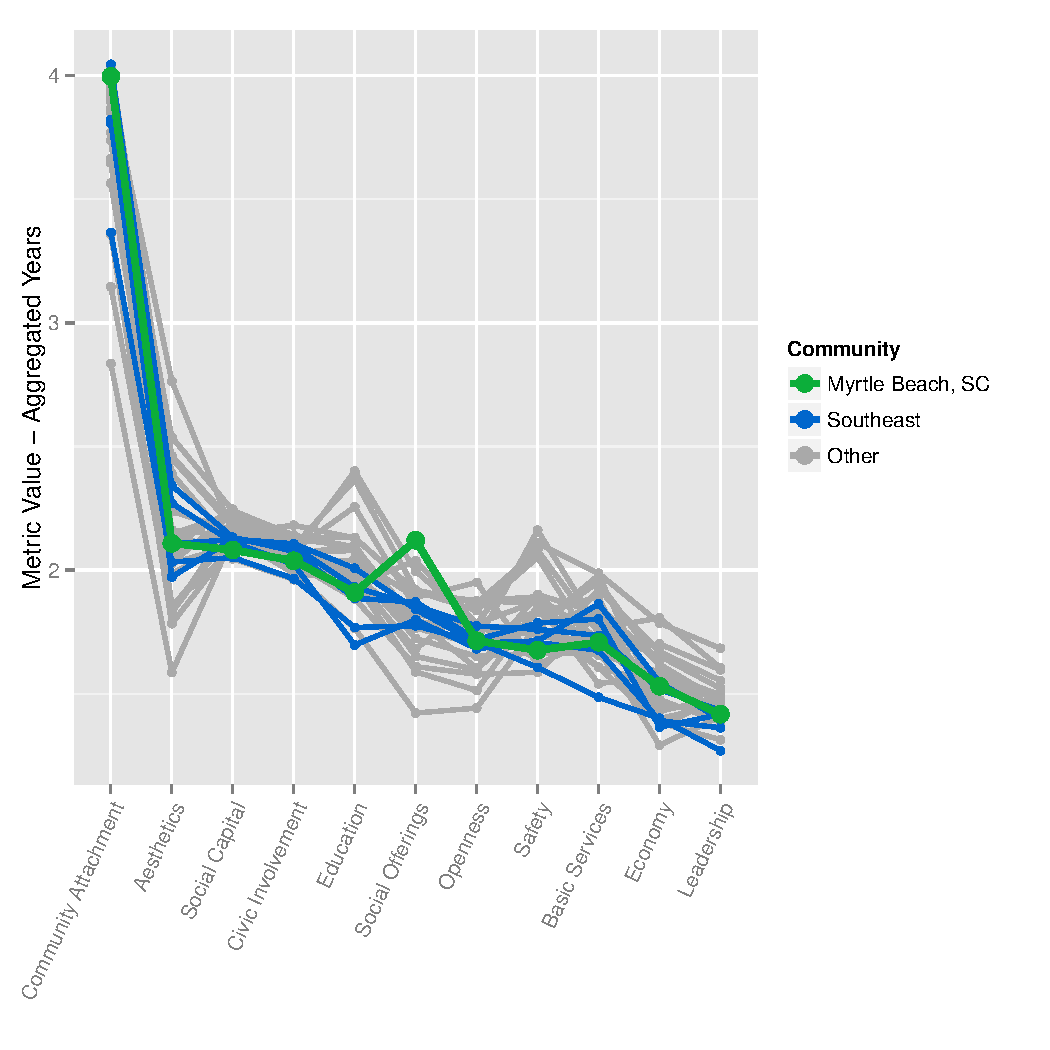
\includegraphics[width=\maxwidth]{figure/southeast_one} 

}

\caption[Mean value of metric for each community]{Mean value of metric for each community. Myrtle Beach is highlighted in green, and the other communities in the Southeast are highlighted in blue.\label{fig:southeast_one}}
\end{figure}


\end{knitrout}


The question remains of how Myrtle Beach has such highly attached citizens when only Social Offerings appears to be a positive metric for the community. The reason is that Social Offerings is the single most highly correlated metric with Community Attachment in 23 out of the 26 communities, including Myrtle Beach.

\subsection{Rust Belt}
As the data covers the period from 2008 to 2010, we hoped to find some stories relating to the economic collapse, or the Great Recession, which began in 2008. We focused on the Economy metric in the Rust Belt communities, and noted a largely negative view of economic conditions in this region, particularly in its economic center, Detroit, MI. Table \ref{tbl:econ} displays the average response on a 1-3 scale for Economy in the Rust Belt communities across each of the three years. It can be seen that although all Rust Belt communities experienced a drop in attitudes about the economy between 2008 and 2009, Detroit's was noticeably smaller. By 2010, attitudes about the economy began to improve. This can also be seen by examining Figure \ref{fig:rb_one}, a density plot of values for Economy in each of the communities in the three years.

% latex table generated in R 3.0.2 by xtable 1.7-1 package
% Thu Feb 13 11:32:27 2014
\begin{table}[ht]
\centering
\begin{tabular}{lrrr}
  \hline
Community & 2008 & 2009 & 2010 \\ 
  \hline
Akron, OH & 1.4135 & 1.3192 & 1.4139 \\ 
  Detroit, MI & 1.2555 & 1.2463 & 1.3718 \\ 
  Fort Wayne, IN & 1.4993 & 1.3572 & 1.5074 \\ 
  Gary, IN & 1.4966 & 1.2803 & 1.3690 \\ 
  Lexington, KY & 1.6949 & 1.5255 & 1.6358 \\ 
  Philadelphia, PA & 1.5965 & 1.4215 & 1.4897 \\ 
  State College, PA & 1.6503 & 1.5914 & 1.7162 \\ 
   \hline
\end{tabular}
\caption{The average value for the Economy metric in the five Rust Belt communities in each of the three years.} 
\label{tbl:econ}
\end{table}



\begin{knitrout}
\definecolor{shadecolor}{rgb}{0.969, 0.969, 0.969}\color{fgcolor}\begin{figure}[H]


{\centering 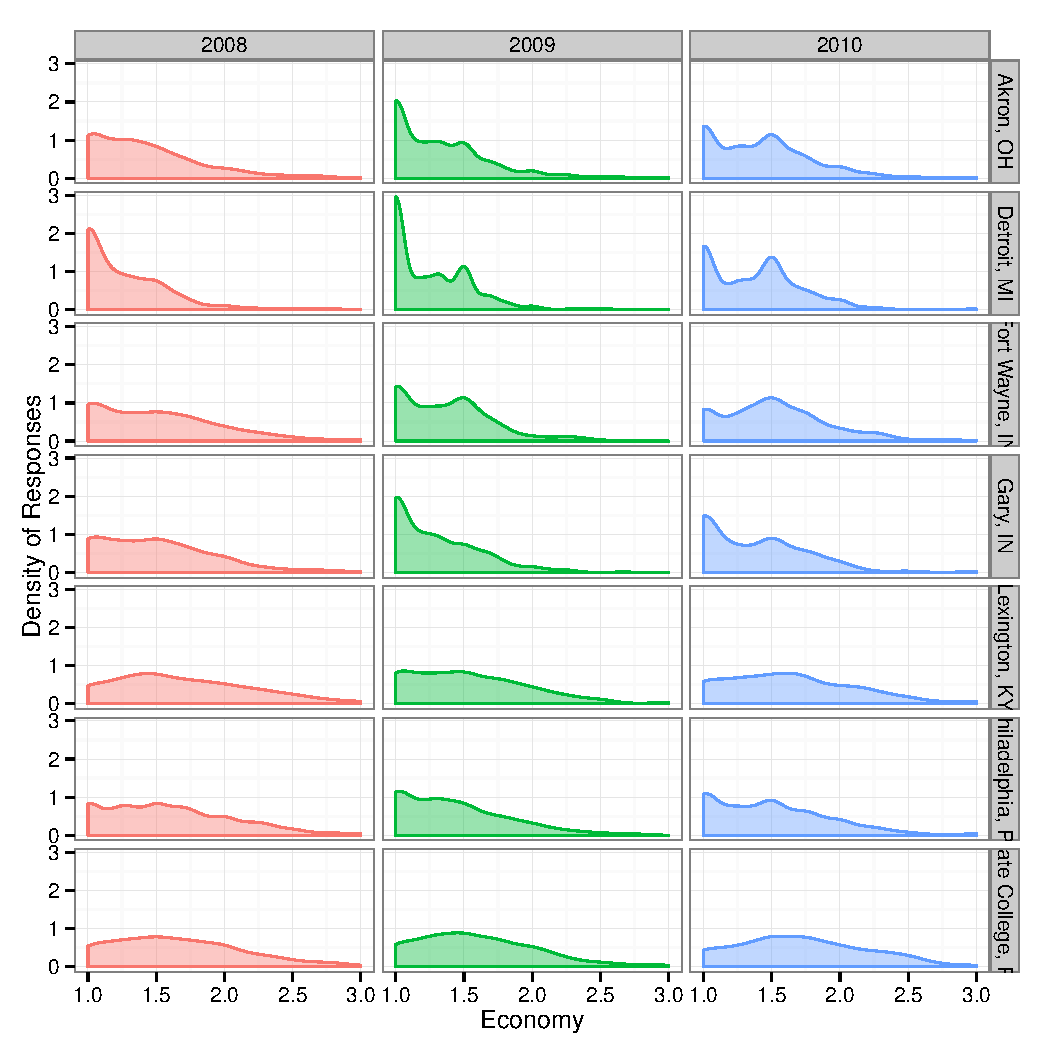
\includegraphics[width=\maxwidth]{figure/rb_one} 

}

\caption[Density of responses in Rust Belt communities over each of the three years]{Density of responses in Rust Belt communities over each of the three years.\label{fig:rb_one}}
\end{figure}


\end{knitrout}


What this table and plot suggests is that although it is widely believed that Detroit was hit especially hard by the economic collapse, there was a bit of resillience in the 2009 and 2010 time frame. Attitudes in Detroit were low regarding the economy in 2008, but did not exhibit much worsening in 2009, and began to improve in 2010. Perhaps the automotive bailouts, which were passed and signed into law in 2009, may be a reasonable explanation for why this occurred in America's ``Motor City".


\section{Conclusion}

The interactive tool, with its use and linked plots and user interaction, allows for the discovery of features and trends in the data that are far more difficult to discover with static plots alone. By creating the tool prior to analyzing the data, we were able to find stories in the data that may not have been as readily apparent otherwise. Specifically, we uncovered an especially strong link between quality of education and Community Attachment in the Great Plains, the importance of Social Offerings in Myrtle Beach and Biloxi, and slowly recovering economic attitudes in the Rust Belt.

While the interactive tool is specialized for this particular dataset, the philosophy and ideas behind its creation hold for other data and applications. By empowering the user to guide his or her own discoveries, the analysis of data can be completed by subject-matter experts in their fields who may be less technologically inclined. The flexibility and ease of Shiny, combined with the interactivity of D3 will hopefully open up a whole new set of possibilities for analyzing complex datasets more easily.


\clearpage

\printbibliography
\end{document}
